\section{Distribuído com Buffers (Assíncrono)}

\subsection{Aplicação assíncrona ao buffer de capacidade finita}
A aplicação assíncrona ao buffer de capacidade finita envolve a utilização de canais assíncronos para gerir o fluxo de dados entre os diferentes módulos do sistema. Esta abordagem permite que o buffer opere de forma eficiente, garantindo que as peças sejam armazenadas e transferidas sem a necessidade de um clock global, o que facilita a coordenação entre os componentes.

Segue na figura abaixo a representação do modelo de rede de Petri com buffers assíncronos.

\begin{figure}[H]
    \centering
    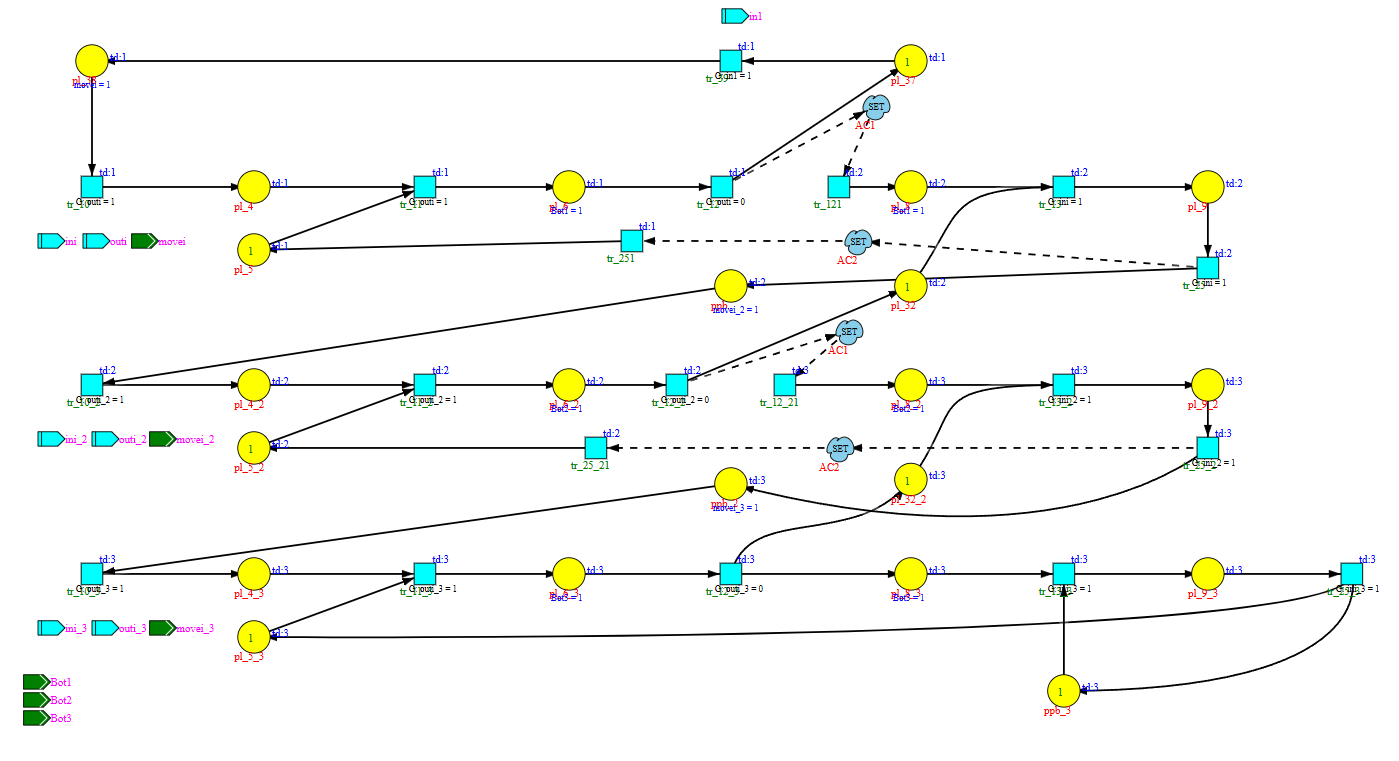
\includegraphics[width=0.8\textwidth]{img/petri_async_channels.png}
    \caption{Rede de Petri - modelo assíncrono com buffers de capacidade finita}\label{fig:petri_async_buffer}
\end{figure}

\subsection{Testes Experimentais}
Os testes experimentais foram realizados para validar o funcionamento do sistema implementado com buffers assíncronos. Os resultados obtidos foram comparados com os resultados da simulação para garantir a consistência e a precisão do modelo.

Neste link tem acesso ao vídeo dos testes experimentais realizados com buffers assíncronos:

\href{https://unlpt-my.sharepoint.com/:v:/g/personal/jafe_lopes_fct_unl_pt/EWEOa2jxXRNFmaCiO5c6iG4BP21vyCbQSKYiZQ8HcoeOrg?nav=eyJyZWZlcnJhbEluZm8iOnsicmVmZXJyYWxBcHAiOiJPbmVEcml2ZUZvckJ1c2luZXNzIiwicmVmZXJyYWxBcHBQbGF0Zm9ybSI6IldlYiIsInJlZmVycmFsTW9kZSI6InZpZXciLCJyZWZlcnJhbFZpZXciOiJNeUZpbGVzTGlua0NvcHkifX0&e=j6h8N4}{Vídeo - Testes experimentais com buffers assíncronos}

Os resultados dos testes demonstraram que o sistema com buffers assíncronos é capaz de operar de forma eficaz, mantendo a integridade dos dados e garantindo a sincronização adequada entre os diferentes módulos, mesmo na ausência de um clock global.

\subsection{Análise comparativa}
%comparar os resultados com async e sync

